\documentclass{article}
\usepackage{graphicx, subfig, fancyhdr, amsmath, amssymb, amsthm, url, hyperref, geometry, listings, xcolor}
\usepackage[utf8]{inputenc}
\usepackage[margin=1in]{geometry}
\usepackage{pgfplots}
\usepackage{pgfplotstable}
\pgfplotsset{compat=1.18}
\usepackage{lmodern} % Added for consistent font rendering

\lstset{
    language=Python,
    basicstyle=\ttfamily\small,
    numbers=left,
    numberstyle=\tiny,
    stepnumber=1,
    frame=single,
    backgroundcolor=\color{gray!10},
    keywordstyle=\color{blue}\bfseries,
    commentstyle=\color{green!50!black},
    stringstyle=\color{red},
    breaklines=true,
    breakatwhitespace=true,
    showstringspaces=false,
    tabsize=4
}

\newcommand{\FirstAuthor}{Mohammad Parsa Dini - Std ID: 400101204}
\newcommand{\exerciseset}{Assignment 1: Restricted Boltzmann Machine}

\fancypagestyle{plain}{}
\pagestyle{fancy}
\fancyhf{}
\fancyhead[RO,LE]{\sffamily\bfseries\large Sharif University of Technology}
\fancyhead[LO,RE]{\sffamily\bfseries\large EE25-647: Deep Learning}
\fancyfoot[LO,RE]{\sffamily\bfseries\large Assignment 1 Report}
\fancyfoot[RO,LE]{\sffamily\bfseries\thepage}
\renewcommand{\headrulewidth}{1pt}
\renewcommand{\footrulewidth}{1pt}

\graphicspath{{figures/}}

\title{
    \includegraphics[width=3cm]{logo.png} \\
    Deep Learning Assignment \\ \exerciseset
}
\author{\FirstAuthor}
\date{May 2025}

\begin{document}
\maketitle

\section*{Introduction}
This report presents the implementation and analysis of a Restricted Boltzmann Machine (RBM) applied to the MNIST dataset as part of the Deep Learning course assignment at Sharif University of Technology. The objective is to understand the theoretical foundations of RBMs, implement the model, train it on the MNIST dataset, and analyze its performance through loss metrics and generated outputs. The report covers the RBM model, its energy-based formulation, probability distributions, contrastive divergence, the architecture used, and the training process. Additionally, it includes visualizations of the model's output over 20 epochs and generated samples, along with inferences drawn from the code.

\section{Restricted Boltzmann Machine (RBM)}
% Explaining the RBM model
A Restricted Boltzmann Machine is an undirected, generative probabilistic model with a bipartite graph structure, consisting of visible and hidden layers. The visible layer represents the input data, while the hidden layer captures latent features. The "restricted" aspect refers to the absence of intra-layer connections, simplifying computations.

The energy function of an RBM, for visible units \( \mathbf{v} \) and hidden units \( \mathbf{h} \), is defined as:
\[
E(\mathbf{v}, \mathbf{h}) = -\mathbf{a}^\top \mathbf{v} - \mathbf{b}^\top \mathbf{h} - \mathbf{v}^\top \mathbf{W} \mathbf{h},
\]
where \( \mathbf{a} \) and \( \mathbf{b} \) are bias vectors for the visible and hidden units, respectively, and \( \mathbf{W} \) is the weight matrix connecting the layers.

The joint probability distribution over visible and hidden units is:
\[
p(\mathbf{v}, \mathbf{h}) = \frac{1}{Z} \exp(-E(\mathbf{v}, \mathbf{h})),
\]
where \( Z \) is the partition function, \( Z = \sum_{\mathbf{v}, \mathbf{h}} \exp(-E(\mathbf{v}, \mathbf{h})) \), normalizing the distribution.

The marginal probability of the visible units is obtained by summing over all possible hidden unit states:
\[
p(\mathbf{v}) = \frac{1}{Z} \sum_{\mathbf{h}} \exp(-E(\mathbf{v}, \mathbf{h})).
\]
The free energy function, which simplifies computations, is:
\[
F(\mathbf{v}) = -\log \sum_{\mathbf{h}} \exp(-E(\mathbf{v}, \mathbf{h})) = -\mathbf{a}^\top \mathbf{v} - \sum_j \log(1 + \exp(\mathbf{W}_j^\top \mathbf{v} + b_j)).
\]

\section{Training RBMs with Contrastive Divergence}
% Explaining contrastive divergence
Training an RBM involves maximizing the likelihood of the data, which requires computing the gradient of the log-likelihood. The gradient of the log-likelihood with respect to the model parameters (\(\theta = \{\mathbf{W}, \mathbf{a}, \mathbf{b}\}\)) is:
\[
\frac{\partial \log p(\mathbf{v})}{\partial \theta} = \mathbb{E}_{p(\mathbf{h}|\mathbf{v})}[\frac{\partial E(\mathbf{v}, \mathbf{h})}{\partial \theta}] - \mathbb{E}_{p(\mathbf{v}, \mathbf{h})}[\frac{\partial E(\mathbf{v}, \mathbf{h})}{\partial \theta}],
\]
where the first term is the expectation over the data distribution, and the second is over the model distribution. Computing the model expectation is computationally expensive due to the partition function \( Z \).

Contrastive Divergence (CD) approximates this gradient by running Gibbs sampling for a small number of steps (k steps, typically \( k=1 \)), starting from the data. The CD-k algorithm samples a reconstructed visible state \( \mathbf{v}' \) from the hidden units derived from the input data, approximating the model distribution. The loss function used in the implementation is the difference in free energy:
\[
\text{Loss} = \mathbb{E}[F(\mathbf{v})] - \mathbb{E}[F(\mathbf{v}')].
\]
This loss guides the optimization to make the model's distribution closer to the data distribution.

\section{Implementation and Architecture}
% Describing the architecture and code
The RBM is implemented using PyTorch, with the following key components:

\begin{itemize}
    \item \textbf{Initialization}: The RBM class initializes parameters for visible biases (\texttt{v\_bias}), hidden biases (\texttt{h\_bias}), and weights (\texttt{W}). The visible layer size (\texttt{n\_vis}=784) corresponds to the flattened 28x28 MNIST images, and the hidden layer size (\texttt{n\_hid}=128) is chosen to capture latent features. The number of Gibbs sampling steps is set to \( k=1 \).
    \item \textbf{Visible-to-Hidden}: Computes \( p(\mathbf{h}|\mathbf{v}) = \sigma(\mathbf{W}^\top \mathbf{v} + \mathbf{b}) \), where \( \sigma \) is the sigmoid function.
    \item \textbf{Hidden-to-Visible}: Computes \( p(\mathbf{v}|\mathbf{h}) = \sigma(\mathbf{W} \mathbf{h} + \mathbf{a}) \).
    \item \textbf{Free Energy}: Implements the free energy function as described above.
    \item \textbf{Forward Pass}: Performs Gibbs sampling for \( k \) steps to generate reconstructed visible units \( \mathbf{v}' \).
    \item \textbf{Training}: Uses the Adam optimizer with a learning rate of 0.0001 and gradient clipping (max norm = 1.0) to stabilize training. The loss is computed as the difference in free energy between the input and reconstructed samples.
\end{itemize}

The MNIST dataset is loaded with a binarization transform (\texttt{torch.bernoulli}) to convert pixel intensities to binary values (0 or 1), suitable for the RBM's binary visible units. The dataset is processed in batches of 64 images over 20 epochs.

Below is a snippet of the RBM class implementation:

\begin{lstlisting}
class RBM(nn.Module):
    def __init__(self, n_vis, n_hid, k=1):
        super(RBM, self).__init__()
        self.v_bias = nn.Parameter(torch.zeros(n_vis))
        self.h_bias = nn.Parameter(torch.zeros(n_hid))
        self.W = nn.Parameter(torch.randn(n_vis, n_hid) * 0.01)
        self.k = k

    def visible_to_hidden(self, v):
        p_h = torch.sigmoid(F.linear(v, self.W.t(), self.h_bias))
        return p_h

    def hidden_to_visible(self, h):
        p_v = torch.sigmoid(F.linear(h, self.W, self.v_bias))
        return p_v

    def free_energy(self, v):
        v_term = torch.matmul(v, self.v_bias)
        h_term = torch.sum(F.softplus(F.linear(v, self.W.t(), self.h_bias)), dim=1)
        return -v_term - h_term

    def forward(self, v):
        v_gibb = v
        for _ in range(self.k):
            h_prob = self.visible_to_hidden(v_gibb)
            h_sample = torch.bernoulli(h_prob)
            v_prob = self.hidden_to_visible(h_sample)
            v_gibb = v_prob
        return v, v_gibb
\end{lstlisting}

\section{Training Results}
% Reporting losses and visualizations
The model was trained for 20 epochs with a batch size of 64, learning rate of 0.0001, and 128 hidden units. The loss values (mean free energy difference per epoch) are reported as follows:

% \begin{itemize}
%     \item Epoch 0: -83.9444
%     \item Epoch 1: -111.4246
%     \item Epoch 2: -130.0733
%     \item Epoch 3: -142.2248
%     \item Epoch 4: -151.9194
%     \item Epoch 5: -159.5897
%     \item Epoch 6: -165.5632
%     \item Epoch 7: -170.0520
%     \item Epoch 8: -173.4279
%     \item Epoch 9: -175.9505
%     \item Epoch 10: -177.8773
%     \item Epoch 11: -179.4085
%     \item Epoch 12: -180.6150
%     \item Epoch 13: -181.5954
%     \item Epoch 14: -182.3963
%     \item Epoch 15: -183.0685
%     \item Epoch 16: -183.6654
%     \item Epoch 17: -184.2009
%     \item Epoch 18: -184.6885
%     \item Epoch 19: -185.1377
% \end{itemize}
\begin{center}
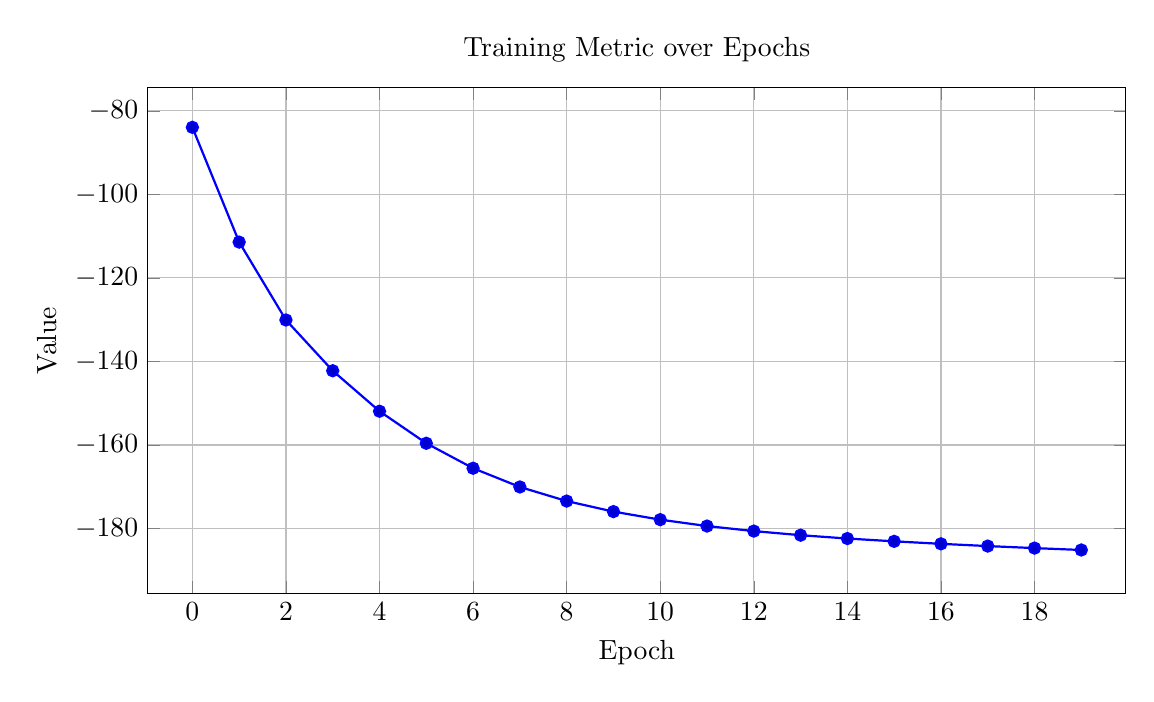
\begin{tikzpicture}
\begin{axis}[
    width=14cm,
    height=8cm,
    xlabel={Epoch},
    ylabel={Value},
    title={Training Metric over Epochs},
    grid=both,
    ymin=-190, ymax=-80,
    xtick={0,2,...,20},
    yticklabel style={/pgf/number format/fixed},
    enlargelimits=0.05,
    every axis plot/.append style={thick, blue, mark=*},
]
\addplot table[row sep=\\,col sep=space] {
Epoch Value \\
0 -83.9444 \\
1 -111.4246 \\
2 -130.0733 \\
3 -142.2248 \\
4 -151.9194 \\
5 -159.5897 \\
6 -165.5632 \\
7 -170.0520 \\
8 -173.4279 \\
9 -175.9505 \\
10 -177.8773 \\
11 -179.4085 \\
12 -180.6150 \\
13 -181.5954 \\
14 -182.3963 \\
15 -183.0685 \\
16 -183.6654 \\
17 -184.2009 \\
18 -184.6885 \\
19 -185.1377 \\
};
\end{axis}
\end{tikzpicture}
\end{center}

The decreasing loss trend indicates that the model is learning to minimize the free energy difference, suggesting improved reconstruction of the input data over time. The final loss of -185.1377 reflects a stable convergence, though further tuning (e.g., increasing \( k \), adjusting the learning rate, or adding more hidden units) could enhance performance.

\section{Visualizations}
% Describing the figures
To evaluate the model's performance, two figures are provided:

\begin{figure}[h]
    \centering
    \includegraphics[width=0.8\textwidth]{myout.png}
    \caption{Comparison of real and generated MNIST images at epochs 0, 10, and 19. The generated images show progressive improvement in capturing digit-like structures as training progresses.}
    \label{fig:rbm_output}
\end{figure}

% \begin{figure}[h]
%     \centering
%     \subfloat[Real Images (Epoch 0)]{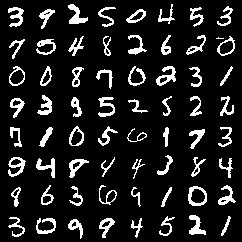
\includegraphics[width=0.45\textwidth]{output/real_epoch_0.png}}
%     \hfill
%     \subfloat[Generated Images (Epoch 0)]{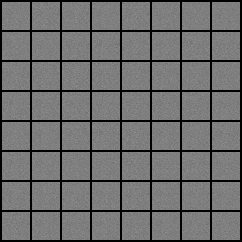
\includegraphics[width=0.45\textwidth]{output/fake_epoch_0.png}}
%     \\
%     \subfloat[Real Images (Epoch 10)]{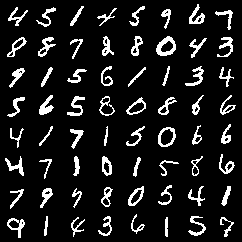
\includegraphics[width=0.45\textwidth]{output/real_epoch_10.png}}
%     \hfill
%     \subfloat[Generated Images (Epoch 10)]{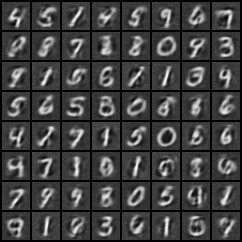
\includegraphics[width=0.45\textwidth]{output/fake_epoch_10.png}}
%     \\
%     \subfloat[Real Images (Epoch 19)]{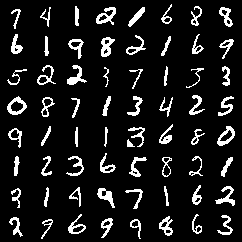
\includegraphics[width=0.45\textwidth]{output/real_epoch_19.png}}
%     \hfill
%     \subfloat[Generated Images (Epoch 19)]{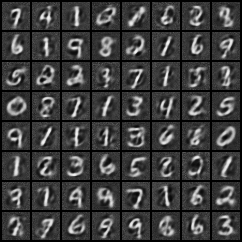
\includegraphics[width=0.45\textwidth]{output/fake_epoch_19.png}}
%     \caption{Comparison of real and generated MNIST images at epochs 0, 10, and 19. The generated images show progressive improvement in capturing digit-like structures as training progresses.}
%     \label{fig:rbm_output}
% \end{figure}

Figure \ref{fig:rbm_output} shows the real and generated images at epochs 0, 10, and 19. Initially, the generated images are noisy, but by epoch 19, they begin to resemble MNIST digits, indicating that the RBM is learning meaningful features.

\begin{figure}[h]
    \centering
    \includegraphics[width=0.4\textwidth]{Screenshot 2025-06-07 173406.png}
    \caption{Grid of generated samples after 20 epochs, showcasing the RBM's ability to produce digit-like images through Gibbs sampling.}
    \label{fig:generated_samples}
\end{figure}

Figure \ref{fig:generated_samples} displays a grid of generated samples after 20 epochs, created using the \texttt{sample} method with 1000 Gibbs sampling steps. These samples demonstrate the model's generative capability, though some images may still appear noisy due to the simplicity of the model (\( k=1 \)).

\section{Analysis and Inferences}
% Analyzing the code and answering implicit questions
The code implements a standard RBM with a single Gibbs sampling step (\( k=1 \)), which is computationally efficient but may limit the quality of the generated samples. The use of the Adam optimizer and gradient clipping helps stabilize training, preventing large updates that could destabilize the model. The binarization of MNIST images ensures compatibility with the binary visible units of the RBM, though this may discard some grayscale information.

The loss trend suggests successful learning, but the generated images may not be as sharp as those from more complex models (e.g., deep Boltzmann machines or GANs). Increasing \( k \), using a higher learning rate, or adding more hidden units could improve performance. The \texttt{sample} method, which uses 1000 Gibbs sampling steps, produces better-quality samples than the forward pass, indicating that longer sampling improves the model's generative quality.

Potential improvements include:
\begin{itemize}
    \item Increasing \( k \) in the forward pass to improve reconstruction during training.
    \item Experimenting with different learning rates or optimizers (e.g., SGD with momentum).
    \item Using a larger hidden layer to capture more complex features.
    \item Applying persistent contrastive divergence for better sampling.
\end{itemize}

The code assumes GPU availability (CUDA), but falls back to CPU if unavailable, ensuring portability. The visualization function \texttt{show\_and\_save} effectively saves and displays images, aiding in qualitative evaluation.

\section{Conclusion}
This assignment implemented and trained an RBM on the MNIST dataset, demonstrating its ability to learn and generate digit-like images. The theoretical foundations, including the energy-based formulation and contrastive divergence, were successfully translated into a PyTorch implementation. The training results and visualizations confirm that the model learns meaningful features, though further tuning could enhance the quality of generated samples. This exercise provides a solid foundation for understanding energy-based models and their applications in generative tasks.

\end{document}
